\subsection{SP4 v4: navegación distribuida hasta el acoplamiento}
\label{subsec:sp4-v4-resultados}

La campaña v4 se mantuvo separada de SP4 v3. Durante desarrollo se detectaron y
corrigieron cuatro fallos que habrían invalidado una conclusión positiva: puertos
geométricamente inalcanzables en el escenario de actuadores, doble conteo de reservas,
violaciones transitorias de capacidad en Euler--replicator y cierre del paso estrecho
por un orden de acoplamiento adverso. Solo después de cerrar esos fallos se congeló el
YAML confirmatorio.

El confirmatorio contiene 60 ejecuciones pareadas: dos semillas no vistas, seis
escenarios, cinco métodos y $N=4$. Las 60 claves
$(\text{semilla},\text{escenario},N,\text{método})$ son únicas. Los gates conjuntos
registraron clearance de puerto mínimo $0{,}10$ m, cero saturaciones físicas de torque,
cero violaciones HOCBF ejecutadas por encima de tolerancia y violación máxima de
capacidad $2{,}22\times10^{-16}$.

\begin{table}[H]
\centering
\caption{SP4 v4 confirmatorio. Cada método tiene 12 mundos pareados.}
\label{tab:sp4-v4-confirmatory}
\small
\begin{tabularx}{\textwidth}{@{}Xrrrrr@{}}
\toprule
Método & Éxito seguro & Colisión & Tiempo (s) & CPU (s) & Capacidad máx. \\
\midrule
Directo + HOCBF & 4/12 & 1/12 & 82{,}82 & 21{,}25 & 0 \\
Prioridad local + HOCBF & 4/12 & 0/12 & 82{,}82 & 10{,}17 & 0 \\
Central + HOCBF & 9/12 & 0/12 & 40{,}20 & 2{,}96 & 0 \\
Replicator distribuido + HOCBF & 12/12 & 0/12 & 25{,}76 & 2{,}18 & $3{,}70\,10^{-17}$ \\
Primal--dual distribuido + HOCBF & 12/12 & 0/12 & 25{,}76 & 2{,}21 & $3{,}70\,10^{-17}$ \\
\bottomrule
\end{tabularx}
\end{table}

\begin{figure}[H]
\centering
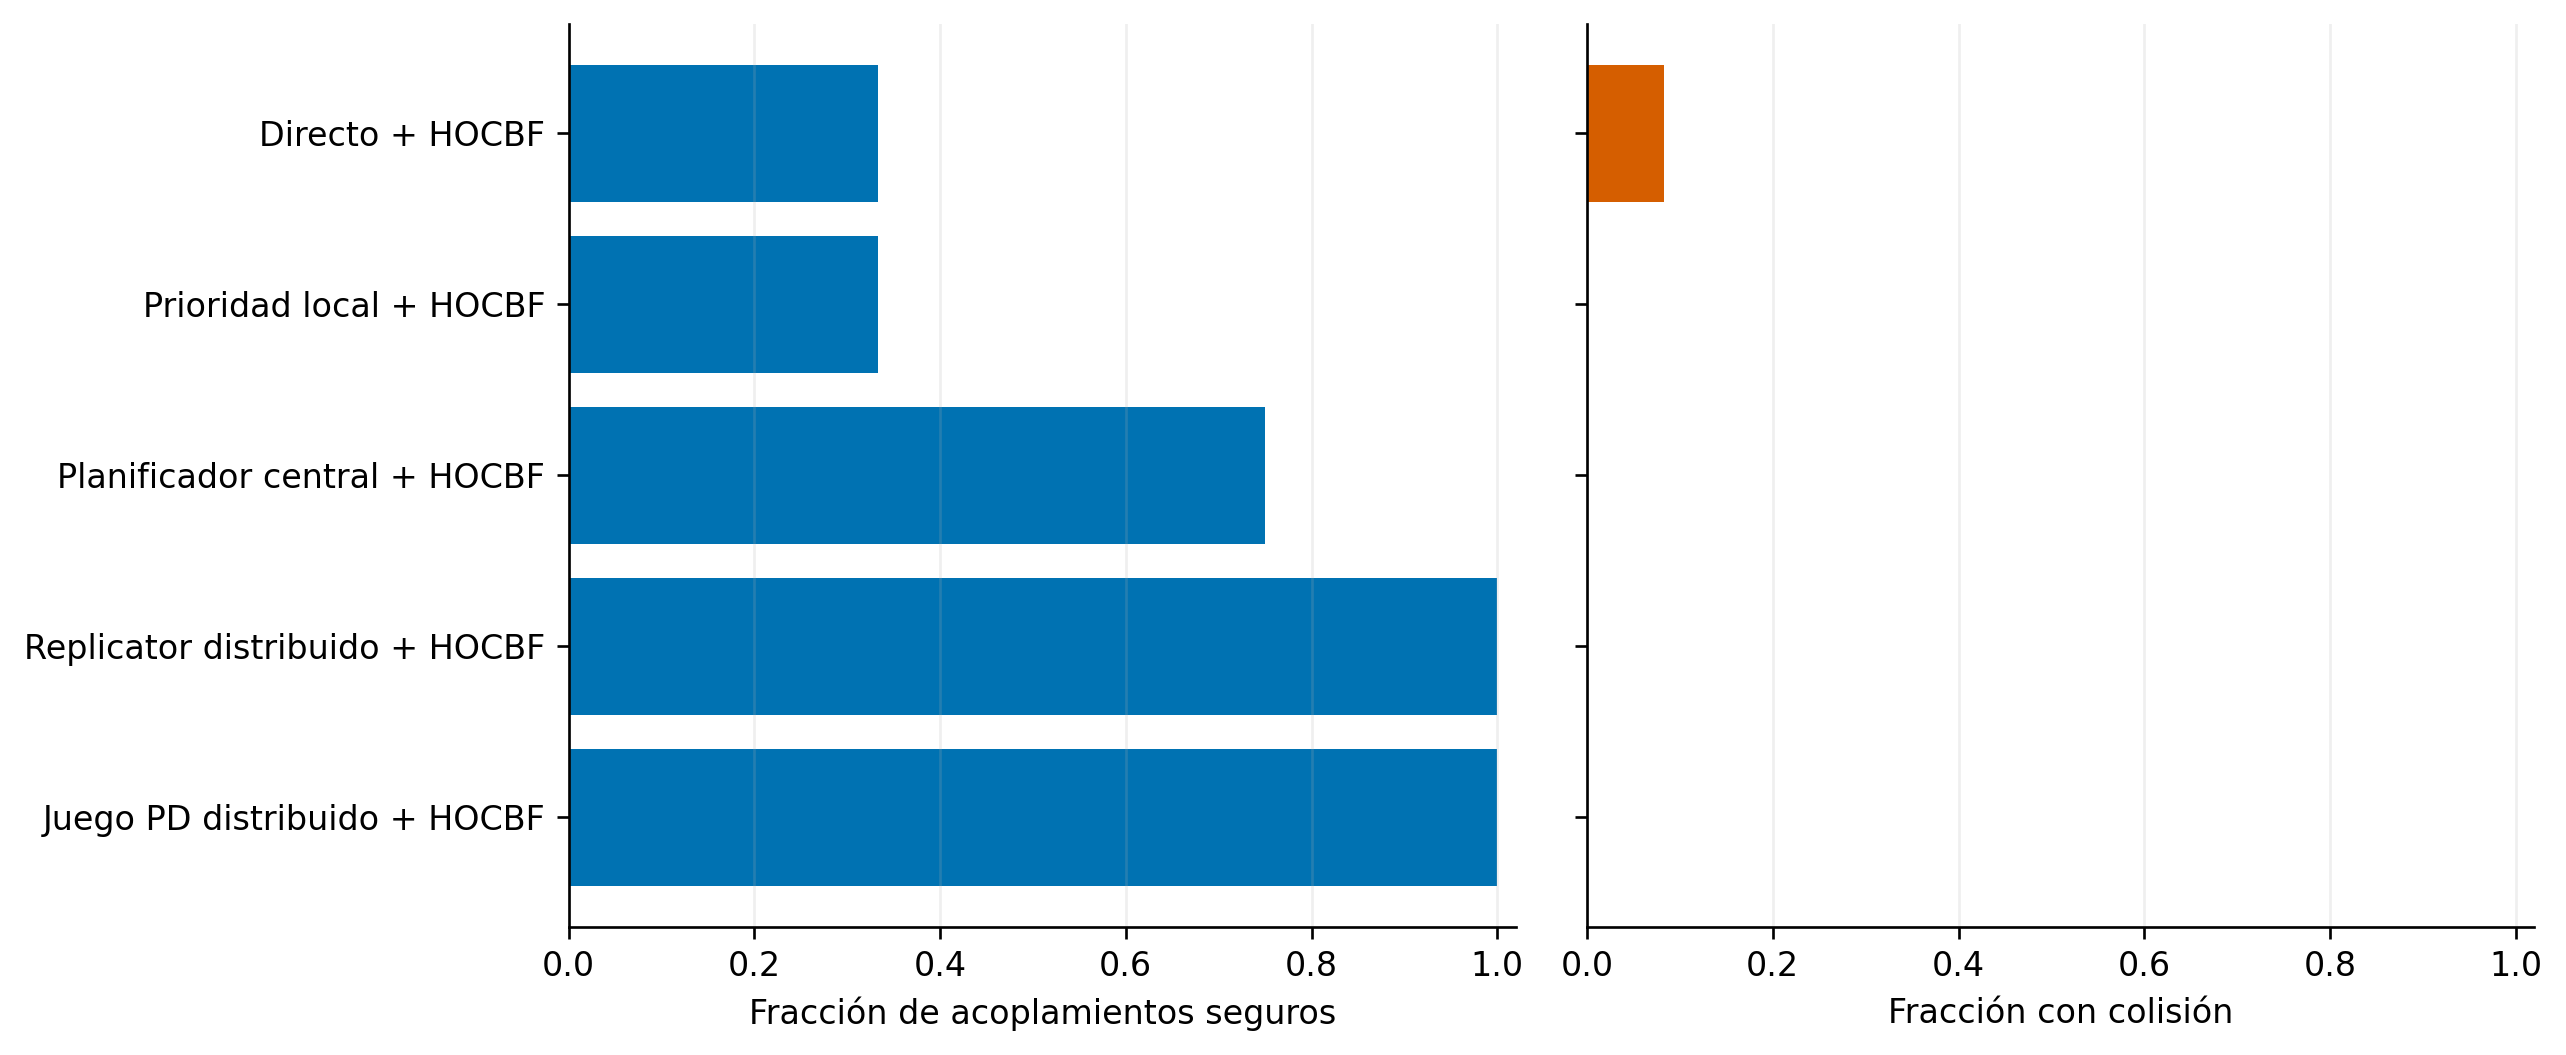
\includegraphics[width=0.94\textwidth]{figures/fig-sp4-v4-performance.png}
\caption{Éxito seguro y colisión en el confirmatorio SP4 v4. El filtro de seguridad no
resuelve por sí mismo los bloqueos de vivacidad.}
\label{fig:sp4-v4-performance}
\end{figure}

PD y replicator ganan ocho pares y no pierden ninguno frente a directo o prioridad; el
test exacto unilateral sobre los ocho pares discordantes da $p=0{,}003906$. Frente a
central solo existen tres pares discordantes, todos a favor del método distribuido, y
$p=0{,}125$. Por tanto, la campaña respalda superioridad sobre los dos baselines locales,
pero no alcanza potencia para declarar superioridad estadística frente a central. PD y
replicator empatan en los 12 mundos; esta campaña no permite preferir uno por éxito.

\begin{figure}[H]
\centering
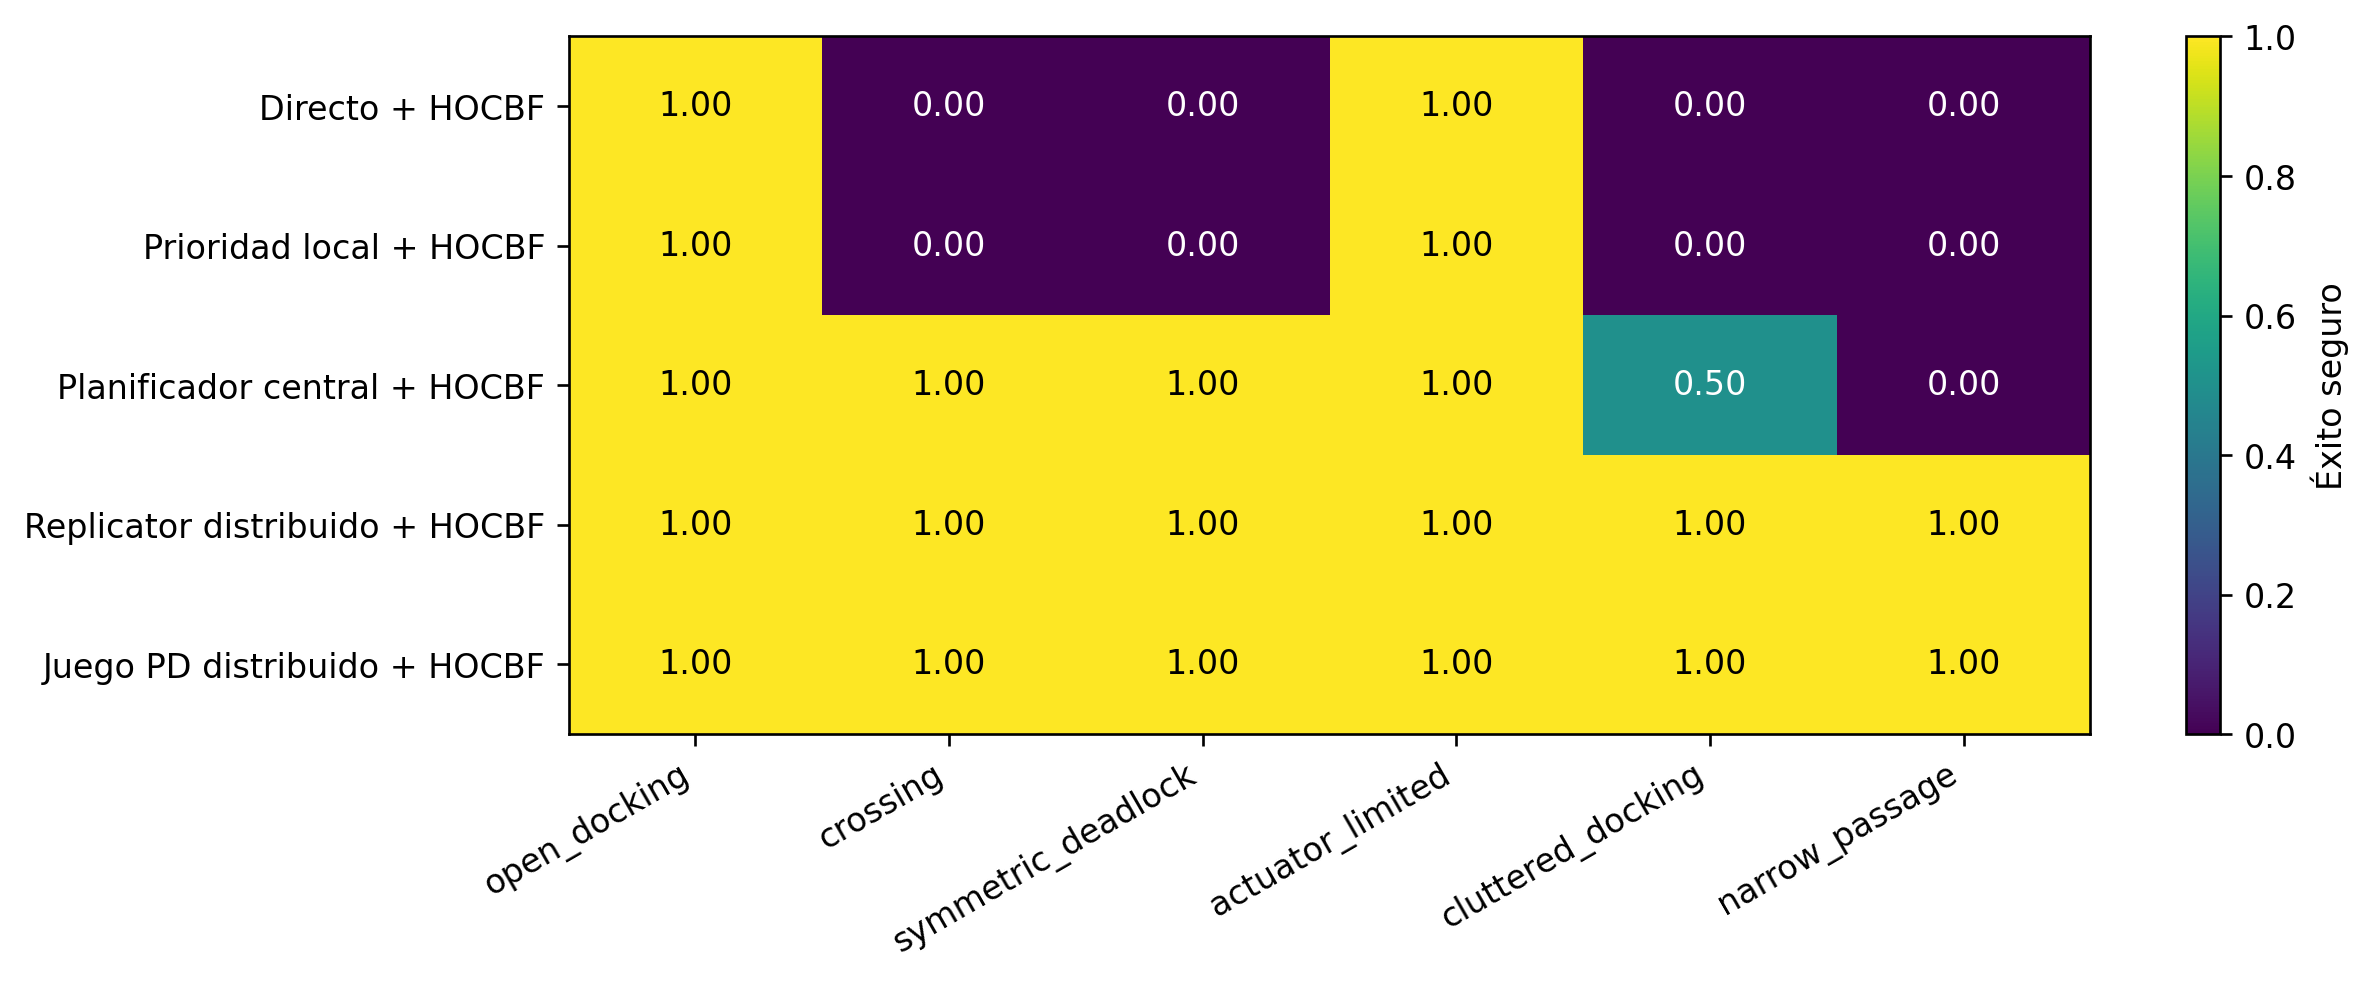
\includegraphics[width=0.96\textwidth]{figures/fig-sp4-v4-scenario-matrix.png}
\caption{Éxito seguro desagregado por escenario. La coloración unitaria en
\texttt{cluttered\_docking} y \texttt{narrow\_passage} prioriza robustez sobre
throughput.}
\label{fig:sp4-v4-matrix}
\end{figure}

La colisión del método directo ocurre en \texttt{narrow\_passage}, semilla 886001, con
clearance mínimo $-5{,}68$ mm. Su residual HOCBF ejecutado permanece por debajo de
$10^{-10}$. Este resultado negativo es importante: la condición diferencial evaluada
antes de integrar no constituye una prueba discreta suficiente. Los métodos propuestos
no colisionan en 24/24 ejecuciones, pero esa cifra es evidencia empírica y no una garantía
universal para cualquier $\Delta t$.

\begin{figure}[H]
\centering
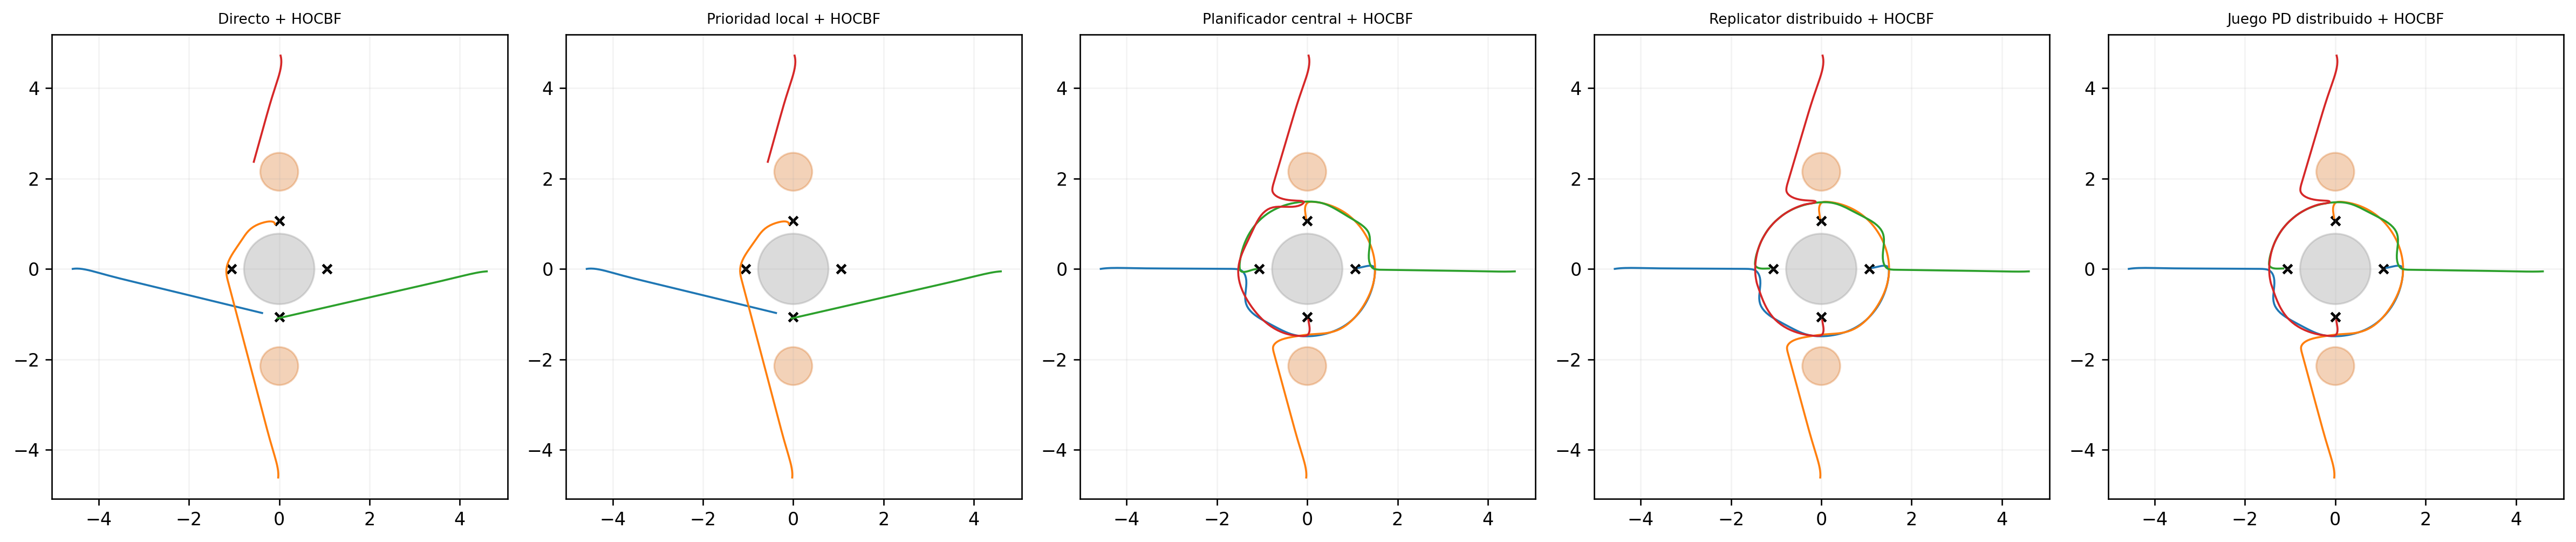
\includegraphics[width=0.98\textwidth]{figures/fig-sp4-v4-trajectories.png}
\caption{Trayectorias representativas en un mundo pareado. Las cruces indican puertos,
el disco gris la carga y los discos naranjas los obstáculos.}
\label{fig:sp4-v4-trajectories}
\end{figure}

El stress test independiente con $N=12$ usa una sola semilla por escenario y no entra en
el contraste anterior. El método primal--dual completa los seis escenarios. En
\texttt{crossing} termina en $85{,}44$ s; en \texttt{cluttered\_docking}, en
$154{,}80$ s; y en \texttt{narrow\_passage}, tras priorización de puertos y
replanificación por fase, en $121{,}92$ s. El último caso mantiene clearance mínimo
$4{,}82$ cm, cero violaciones ejecutadas, cero saturaciones y capacidad cero, pero consume
$113{,}06$ s de CPU. Así, la factibilidad escala mejor que la eficiencia de esta
implementación secuencial.

\begin{figure}[H]
\centering
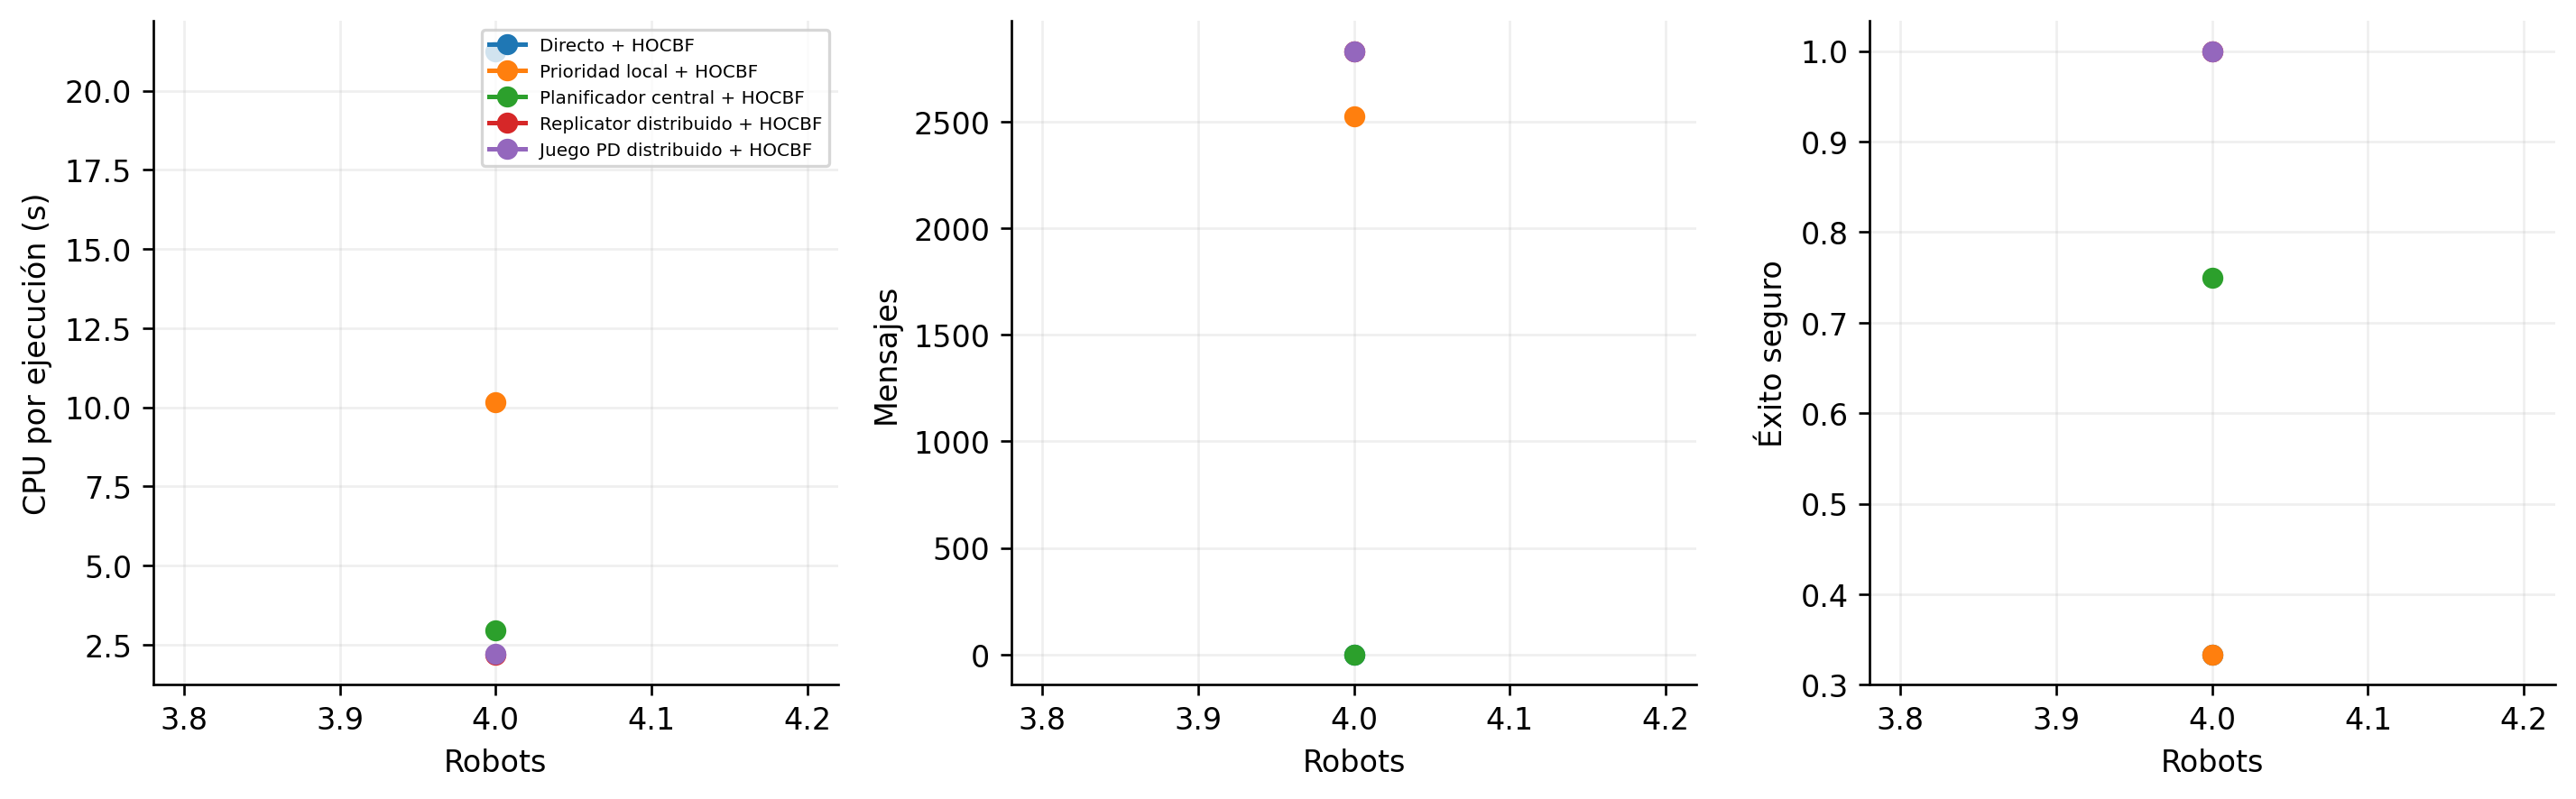
\includegraphics[width=0.88\textwidth]{figures/fig-sp4-v4-scaling.png}
\caption{Métricas de escalabilidad producidas por el ejecutor v4. La figura confirmatoria
solo contiene $N=4$; los valores N=12 se reportan como certificados de stress separados.}
\label{fig:sp4-v4-scaling}
\end{figure}

\subsubsection{Validación visual pareada en CoppeliaSim}
La escena autocontenida \texttt{sp4\_v4\_paired\_narrow\_passage.ttt} se ejecutó en el
motor real de CoppeliaSim, sin render sintético de sustitución. Contiene dos copias del
mismo mundo, ocho Pioneer y 690 objetos, y exportó 29 capturas. La izquierda reproduce
directo+HOCBF; la derecha, primal--dual+HOCBF. El error máximo entre poses ordenadas y
medidas por CoppeliaSim fue $6{,}89\times10^{-9}$ m. En el lado directo se recuperó la
penetración de $-5{,}68$ mm y el fallo de llegada; en el propuesto se midió clearance
mínimo $5{,}71$ cm y acoplamiento seguro. Por diseño, se trata de reproducción
cinemática del controlador ya evaluado: refuerza validez geométrica y trazabilidad
visual, pero no constituye una validación dinámica independiente.

\begin{figure}[H]
\centering
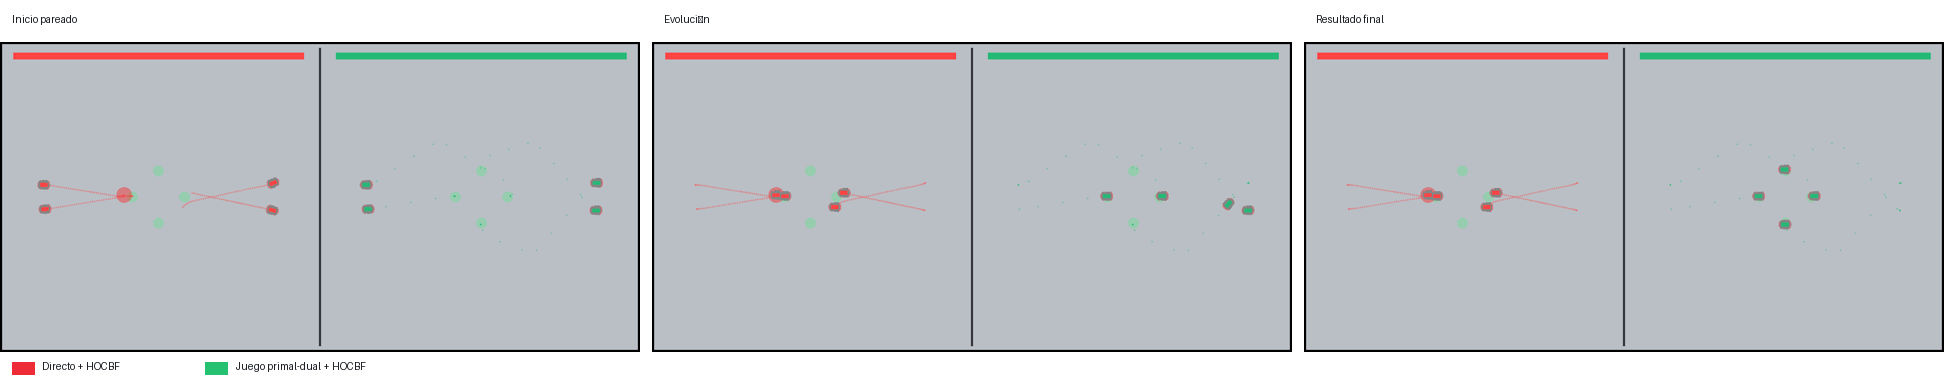
\includegraphics[width=\textwidth]{figures/fig-sp4-v4-coppelia-paired.png}
\caption{Escena pareada SP4 v4 en CoppeliaSim. Cada panel temporal contiene el baseline
directo (izquierda, rojo) y el juego primal--dual (derecha, verde) bajo idéntica
geometría y semilla. El baseline queda bloqueado tras la colisión; el método propuesto
alcanza los cuatro puertos.}
\label{fig:sp4-v4-coppelia-paired}
\end{figure}

La conclusión defendible es acotada. En los mundos confirmatorios N=4, añadir el juego y
la clausura de vivacidad al mismo filtro HOCBF eleva el éxito de 4/12 (local) y 9/12
(central) a 12/12. El aporte no es una nueva garantía total de planificación
multi-robot: depende de A*, factibilidad de puertos, coloración conservadora y
replanificación. Tampoco se ha validado aún con ORCA real, un lazo dinámico independiente en CoppeliaSim
o hardware para SP4 v4. Esos tres elementos quedan como trabajo necesario antes de
afirmar madurez robótica completa.